%%%%%%%%%%%%%%%%%%%%%%%%%%%%%%%%%%%%%%%%%
% Jacobs Landscape Poster
% LaTeX Template
% Version 1.1 (14/06/14)
%
% Created by:
% Computational Physics and Biophysics Group, Jacobs University
% https://teamwork.jacobs-university.de:8443/confluence/display/CoPandBiG/LaTeX+Poster
%
% Further modified by:
% Nathaniel Johnston (nathaniel@njohnston.ca)
%
% This template has been downloaded from:
% http://www.LaTeXTemplates.com
%
% License:
% CC BY-NC-SA 3.0 (http://creativecommons.org/licenses/by-nc-sa/3.0/)
%
%%%%%%%%%%%%%%%%%%%%%%%%%%%%%%%%%%%%%%%%%

%----------------------------------------------------------------------------------------
%	PACKAGES AND OTHER DOCUMENT CONFIGURATIONS
%----------------------------------------------------------------------------------------

\documentclass[xcolor=table,final]{beamer}

\usepackage[scale=1.15]{beamerposter} % Use the beamerposter package for laying out the poster


\usetheme{confposter} % Use the confposter theme supplied with this template

\setbeamercolor{block title}{fg=jblue,bg=white} % Colors of the block titles
\setbeamercolor{block body}{fg=black,bg=white} % Colors of the body of blocks
\setbeamercolor{block alerted title}{fg=white,bg=dblue!70} % Colors of the highlighted block titles
\setbeamercolor{block alerted body}{fg=black,bg=dblue!10} % Colors of the body of highlighted blocks
% Many more colors are available for use in beamerthemeconfposter.sty

%-----------------------------------------------------------
% Define the column widths and overall poster size
% To set effective sepwid, onecolwid and twocolwid values, first choose how many columns you want and how much separation you want between columns
% In this template, the separation width chosen is 0.024 of the paper width and a 4-column layout
% onecolwid should therefore be (1-(# of columns+1)*sepwid)/# of columns e.g. (1-(4+1)*0.024)/4 = 0.22
% Set twocolwid to be (2*onecolwid)+sepwid = 0.464
% Set threecolwid to be (3*onecolwid)+2*sepwid = 0.708

\newlength{\sepwid}
\newlength{\onecolwid}
\newlength{\twocolwid}
\newlength{\threecolwid}
\setlength{\paperwidth}{46.8in} % A0 width: 46.8in
\setlength{\textwidth}{44.8in}
\setlength{\paperheight}{33.1in} % A0 height: 33.1in
\setlength{\textwidth}{31.1in}
\setlength{\sepwid}{0.024\paperwidth} % Separation width (white space) between columns
\setlength{\onecolwid}{0.22\paperwidth} % Width of one column
\setlength{\twocolwid}{0.464\paperwidth} % Width of two columns
\setlength{\threecolwid}{0.708\paperwidth} % Width of three columns
\setlength{\topmargin}{-0.5in} % Reduce the top margin size

%-----------------------------------------------------------


\usepackage{booktabs} % Top and bottom rules for tables

\makeatletter
\let\@@magyar@captionfix\relax
\makeatother

\usepackage{graphicx}
\usepackage{subfig}

% Matrix decomposition diagram
\usepackage{stackengine}
\stackMath
\newlength\matfield
\newlength\tmplength
\def\matscale{1.}
\newcommand\dimbox[3]{%
  \setlength\matfield{\matscale\baselineskip}%
  \setbox0=\hbox{\vphantom{X}\smash{#3}}%
  \setlength{\tmplength}{#1\matfield-\ht0-\dp0}%
  \fboxrule=1pt\fboxsep=-\fboxrule\relax%
  \fbox{\makebox[#2\matfield]{\addstackgap[.5\tmplength]{\box0}}}%
}
\newcommand\raiserows[2]{%
   \setlength\matfield{\matscale\baselineskip}%
   \raisebox{#1\matfield}{#2}%
}
\newcommand\matbox[5]{
  \stackunder{\dimbox{#1}{#2}{$#5$}}{\scriptstyle(#3\times #4)}%
}
\parskip 1em

\usepackage{siunitx} % For scientific notation of p-values using \num

\usepackage{tabularx}
% Tables with merged vertical cells
\usepackage{multirow}

\setbeamerfont{block title}{size=\LARGE}
\setbeamerfont{caption}{size=\footnotesize}

% set colors for alerted blocks (blocks with frame)
\setbeamercolor{block alerted title}{fg=white,bg=nred}
\setbeamercolor{block alerted body}{fg=black,bg=nred!10}

\renewcommand{\bold}[1]{{\textcolor{norange}{\textbf{#1}}}}

%----------------------------------------------------------------------------------------
%	TITLE SECTION
%----------------------------------------------------------------------------------------

\newcommand{\samelineand}{\qquad}

\title{Comparison of sparse biclustering algorithms for gene expression datasets} % Poster title
\author[shortname]{Katherine Nicholls \inst{1} \inst{2} and Chris Wallace \inst{1} \inst{2}}

\institute[shortinst]{\inst{1} Cambridge Institute for Therapeutic Immunology and Infectious Disease, University of Cambridge, Cambridge, CB2 0AW, UK \inst{2} MRC Biostatistics Unit, Cambridge Biomedical Campus, Forvie Site, Robinson Way, Cambridge, CB2 0SR, UK}

%----------------------------------------------------------------------------------------

\begin{document}

\addtobeamertemplate{block end}{}{\vspace*{2ex}} % White space under blocks
\addtobeamertemplate{block alerted end}{}{\vspace*{2ex}} % White space under highlighted (alert) blocks

%\setlength{\belowcaptionskip}{2ex} % White space under figures
\setlength\belowdisplayshortskip{2ex} % White space under equations


\begin{frame}[t] % The whole poster is enclosed in one beamer frame

\begin{columns}[t] % The whole poster consists of three major columns, the second of which is split into two columns twice - the [t] option aligns each column's content to the top

\begin{column}{\sepwid}\end{column} % Empty spacer column

\begin{column}{\onecolwid} % The first column

%----------------------------------------------------------------------------------------
%	INTRODUCTION
%----------------------------------------------------------------------------------------

\begin{block}{Why biclustering?}

Biclusters: groups of \bold{genes that covary} in a \bold{subset of the samples}.

\begin{itemize}
    \item Detects patterns not visible with gene clustering
    \item Provides link between samples and gene groups
    \item Adjusts for confounders
\end{itemize}

\begin{figure}
    \captionsetup[subfigure]{justification=centering}
\begin{minipage}{1\linewidth}
    \centering
\subfloat[Original matrix \label{fig:raw}]{
    
\includegraphics[width=0.2\textwidth]{plots/biclustering_diagrams/raw.png}}
\subfloat[Clustering genes\label{fig:rows}]{
    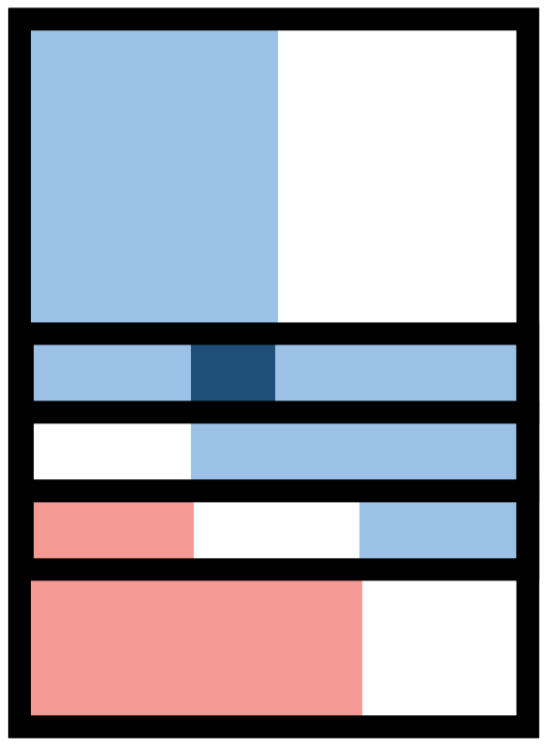
\includegraphics[width=0.2\textwidth]{plots/biclustering_diagrams/rows.png}}
\subfloat[Clustering samples\label{fig:cols}]{
    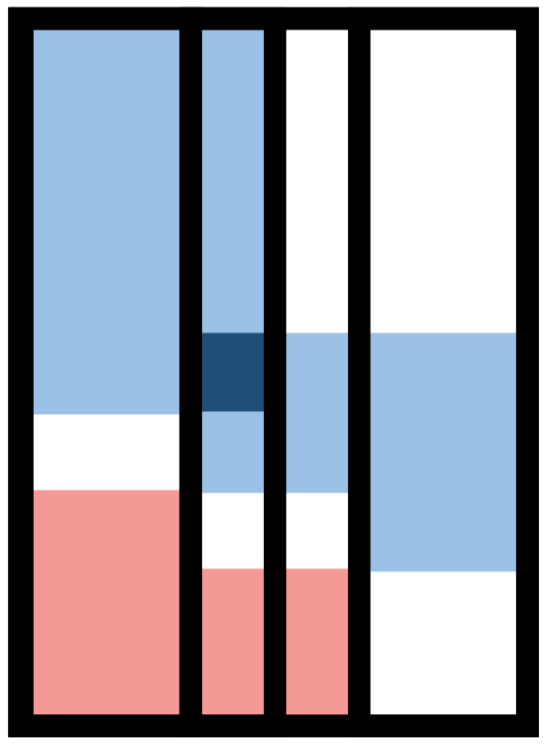
\includegraphics[width=0.2\textwidth]{plots/biclustering_diagrams/cols.png}}
\end{minipage}
\\
\begin{minipage}{1\linewidth}
    \centering
\subfloat[Biclustering\label{fig:biclusters}]{
    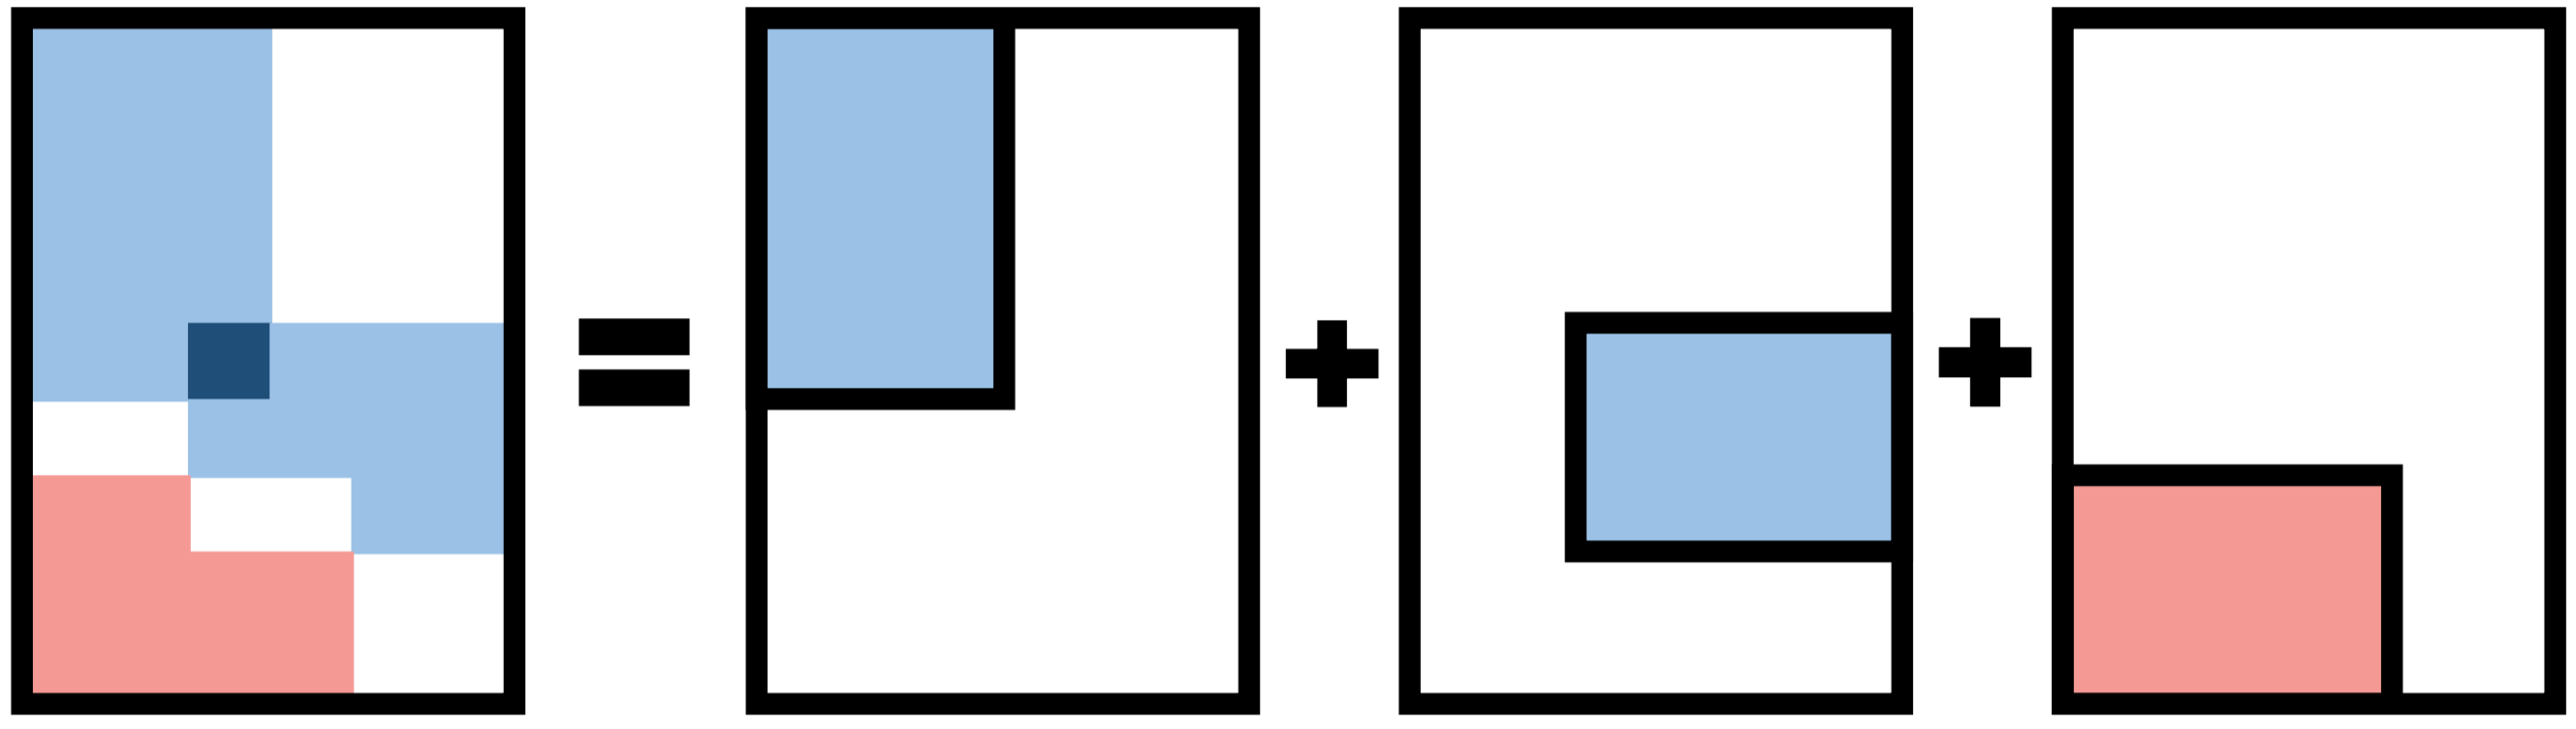
\includegraphics[width=0.85\textwidth]{plots/biclustering_diagrams/biclusters.png}}
\end{minipage}
\caption{The same matrix is used for each type of clustering, with rows as genes and columns as samples. Only biclustering captures the true structure of the dataset.}
\label{fig:caption}
    \end{figure}

\end{block}

%------------------------------------------------

%----------------------------------------------------------------------------------------
%	ALGORITHMS
%----------------------------------------------------------------------------------------

\begin{block}{Algorithm classes}

\begin{table}[t!]
    \caption{Overview of the four classes of biclustering algorithm included.}

    \begin{tabular}{ l | l }
\textbf{Class} & \textbf{Advantages} \\ \hline
\cellcolor[HTML]{50bd4c}\color[HTML]{FFFFFF}\textbf{\textit{Popular}} & \multirow{2}{0.55 \textwidth}{Benchmark - in previous comparison studies} \\
     FABIA, Plaid & \\ \hline
    \cellcolor[HTML]{3B93DC}\color[HTML]{FFFFFF}\textbf{\textit{NMF}} & \multirow{2}{0.55 \textwidth}{Fast, interpretable} \\
    nsNMF, SNMF & \\ \hline
    \cellcolor[HTML]{7f1c8e}\color[HTML]{FFFFFF}\textbf{\textit{Tensor}} & \multirow{2}{0.55 \textwidth}{Share information across cell types} \\
    MultiCluster, SDA & \\ \hline
    \cellcolor[HTML]{C50F11}\color[HTML]{FFFFFF}\textbf{\textit{Adaptive}} & \multirow{2}{0.55 \textwidth}{Mixture of sparse and dense factors, learn K automatically} \\
    BicMix, SSLB & \\ \hline
\end{tabular}
\end{table}

\end{block}


%----------------------------------------------------------------------------------------
%	Study aims
%----------------------------------------------------------------------------------------


\begin{block}{Novel study features}

\begin{itemize}
    \item \bold{Algorithm classes} not previously compared
    \item \bold{Range of complexity} of simulated datasets
    \item \bold{Direct evaluation} of biclustering on \bold{real datasets}
\end{itemize}

\end{block}

%----------------------------------------------------------------------------------------




\end{column} % End of the first column

\begin{column}{\sepwid}\end{column} % Empty spacer column

\begin{column}{\twocolwid} % The second column (double column)

%----------------------------------------------------------------------------------------
%	RESULTS
%----------------------------------------------------------------------------------------

\begin{block}{Results}
\end{block}

% Split this middle column into two
\begin{columns}
\begin{column}{\onecolwid}

\begin{figure}
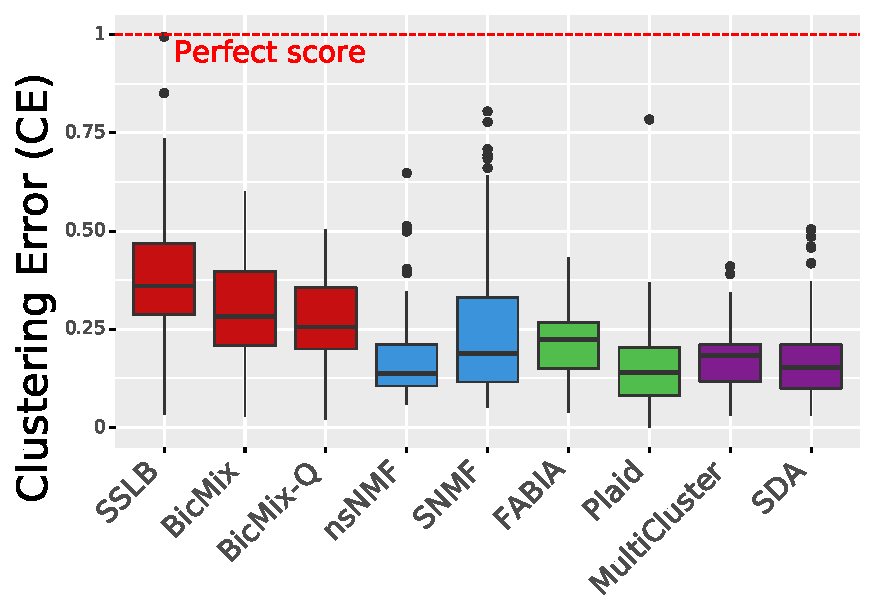
\includegraphics[width=0.9 \textwidth]{plots/summary_clust_err_best_theoretical_K_init.pdf}
\caption{Caption}
\end{figure}

\begin{figure}
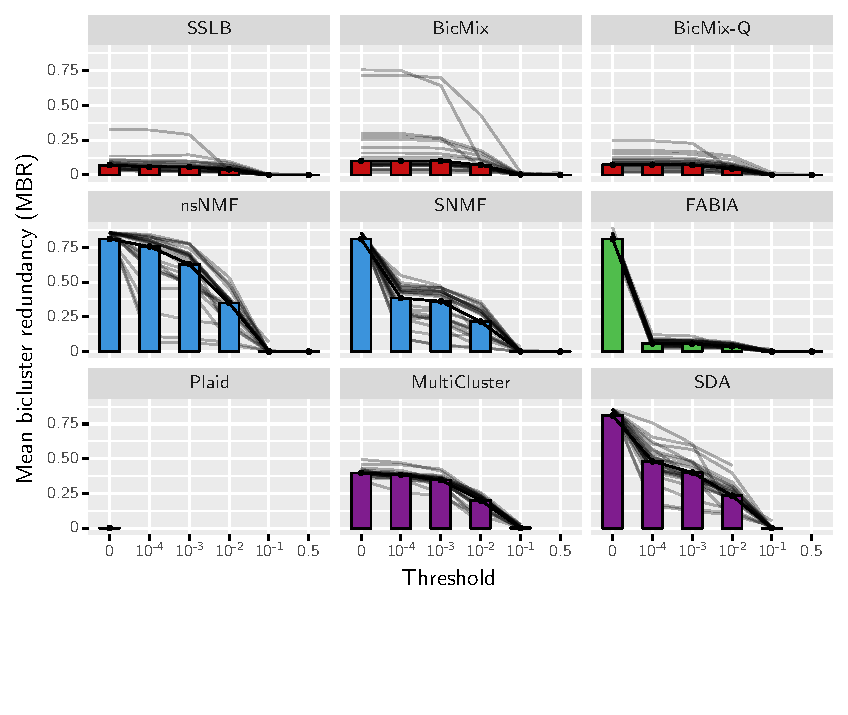
\includegraphics[width=0.9 \textwidth]{plots/threshold_adjusted_redundancy_mean_lines.pdf}
\caption{Caption}
\end{figure}

\begin{figure}
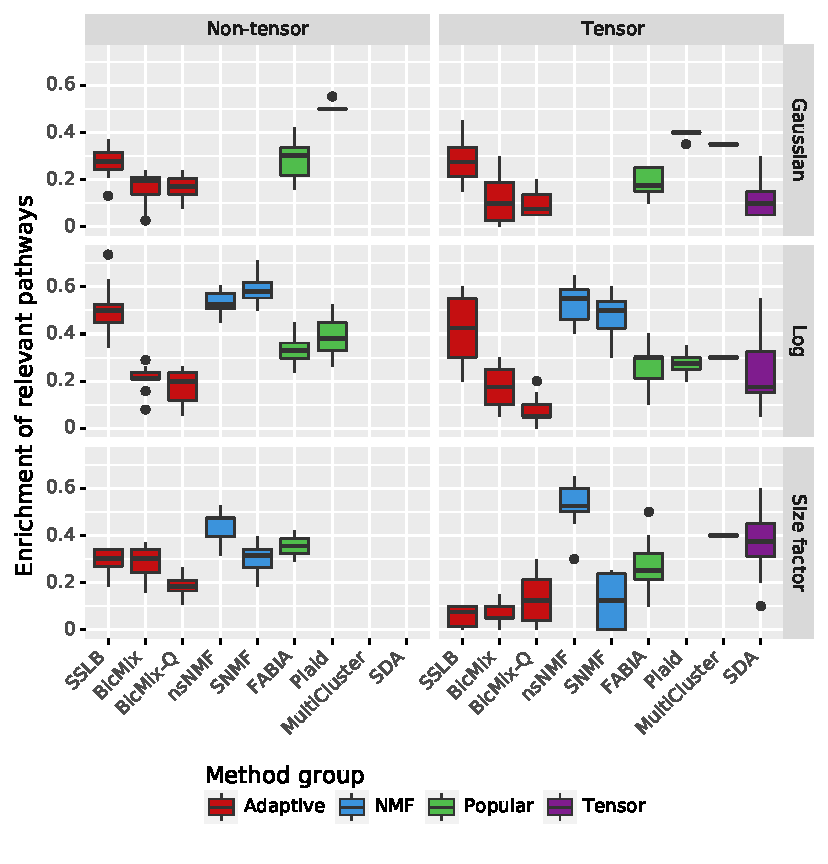
\includegraphics[width=0.9 \textwidth]{plots/compare_samegenes_K_50_datasets_ko_traits_nz_alpha_0-05.pdf}
\caption{Caption}
\end{figure}

\end{column} % End of column 2.1

\begin{column}{\onecolwid} % The third column

\begin{figure}
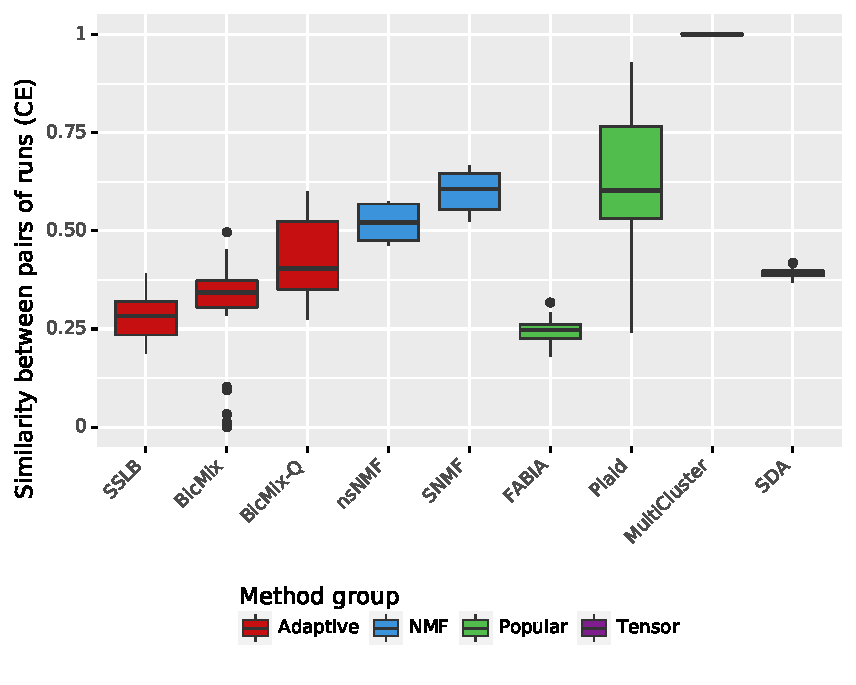
\includegraphics[width=0.9 \textwidth]{plots/similarity_methods_K.pdf}
\caption{Caption}
\end{figure}

\begin{figure}
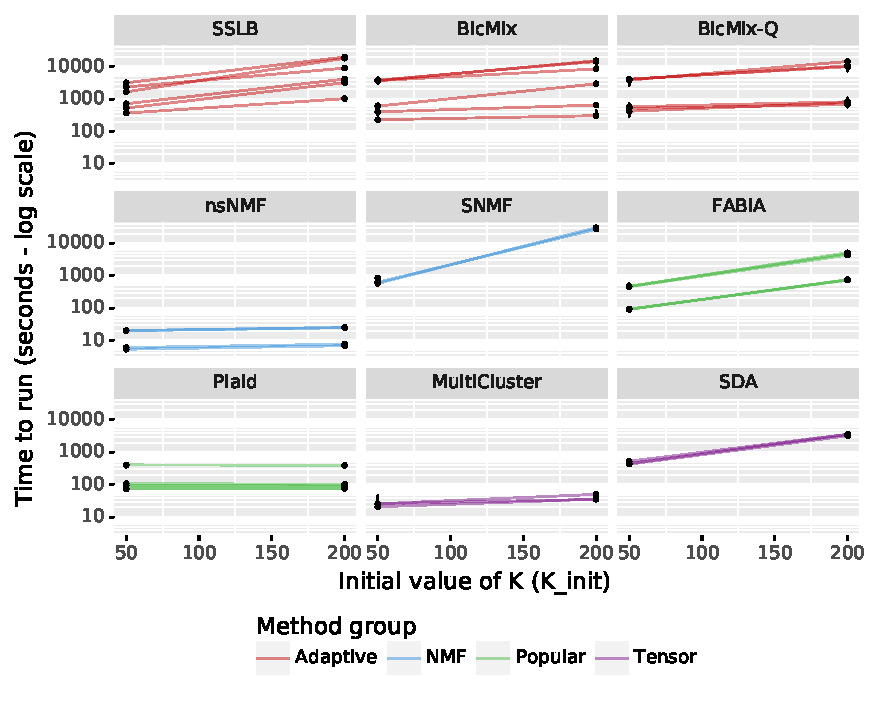
\includegraphics[width=0.9 \textwidth]{plots/IMPC_comp_reqs_s_against_K.pdf}
\caption{Caption}
\end{figure}

\end{column} % End of column 2.2
\end{columns} % End of two columns comprising middle column

%----------------------------------------------------------------------------------------

\end{column} % End of middle (double) column

\begin{column}{\sepwid}\end{column} % Empty spacer column
\begin{column}{\onecolwid} % The fourth column

%----------------------------------------------------------------------------------------
%	CONCLUSION
%----------------------------------------------------------------------------------------

\begin{block}{Conclusion}

\begin{itemize}
    \item Post-processing thresholding essential for most algorithms
    \item Adaptive algorithms best on dataset with unknown K and without processing
    \item NMF algorithms have potential - fast, robust and nsNMF performed well
    \item Little benefit found for tensor algorithms
    \item Introduced metrics for real datasets where truth is not known
\end{itemize}

\end{block}

\begin{alertblock}{Preprint}
For more details, see the preprint on bioRxiv: \\
\small \url{https://doi.org/10.1101/2020.12.15.422852}
\end{alertblock}

%----------------------------------------------------------------------------------------
%	REFERENCES
%----------------------------------------------------------------------------------------

\begin{block}{References}

\nocite{*} % Insert publications even if they are not cited in the poster
{\bibliographystyle{plain}
\bibliography{poster}}

\end{block}

%----------------------------------------------------------------------------------------
%	ACKNOWLEDGEMENTS
%----------------------------------------------------------------------------------------

\begin{center}
\begin{tabular}{ccccc}

\includegraphics[height=22mm]{./Cambridge_University_CMYK.eps} & \hspace{15mm} & 
\includegraphics[height=22mm]{mrc_logo.jpg} & \hspace{15mm} & 
\includegraphics[height=22mm]{wellcome-logo-black.jpg}
\end{tabular}
\end{center}

%----------------------------------------------------------------------------------------

\end{column} % End of the fourth column

\end{columns} % End of all the columns in the poster

\end{frame} % End of the enclosing frame

\end{document}
